%\documentclass[10pt,fleqn]{article}
%\documentclass[letterpaper,10pt,fleqn]{article}
\documentclass[twoside,twocolumn,10pt,fleqn]{article}
\usepackage[margin=1in,footskip=0.25in]{geometry}
\usepackage{amsmath}
\usepackage{amsthm}
\usepackage{amsfonts}
\usepackage{amssymb}
\renewcommand{\theequation}{\arabic{equation}}
\usepackage[ruled]{algorithm2e}
\usepackage{tikz}

\title{A Byzantine Fault-tolerant Key-value Store}
\author{Ryuji Ishiguro}
\date{\today}

\usepackage{titling} % Customizing the title section
\usepackage{abstract} % Allows abstract customization
\renewcommand{\maketitlehookd}{%
\begin{abstract}
  \noindent
  Most distributed key-value stores are tolerant to only benign failure,
  which makes it difficult to run it on the public Internet and needs
  additional security measures to protect data integrity from malicious
  attacks. We developed a key-value store that is tolerant to Byzantine
  faults, keeping it in mind to run the system over the public
  Internet. While data integrity is secured on the store, all
  transactions are transparent to anyone.
  The system provides not only data integrity but also data secrecy by
  strong password authentication, encryption and signature schemes
  based on threshold cryptography. Integrating encryption and
  signature schemes with Byzantine tolerant key-value store is much
  more robust than using separated KMS and PKI with an ordinary
  distributed key-value store, as it maximizes a benefit of distributed
  system which fits very well with threshold cryptography. There is no
  single point of failure in the system.
  The system by itself is useful as a secure key-value store, but those
  properties such as Byzantine fault-tolerance, transparency,
  distributed global storage and threshold cryptography, can make the
  system a building block of blockchain technologies.
\end{abstract}
}

\begin{document}

\maketitle

\section{Introduction}
How to reach a consensus with Byzantine type failure is the main
problem of blockchain technologies. Bitcoin blockchain uses PoW with
incentives \cite{bitcoin}. Majority of public blockchain (or permission-less
blockchain) has the same type of consensus mechanism. Another type of
consensus mechanism is to use BFT protocols, which is a major
mechanism for local/enterprise blockchain (or permissioned
system). Some PoS type blockchain technologies use BFT as well to
improve the transaction rate.

The proposed system is based on the Byzantine quorum system introduced
by Malhi and Reiter \cite{Delhi:1}. We construct a $b$-masking quorum
system based on Web of Trust graph. We also introduce quorum certificates
combined with a threshold authentication scheme to protect data from
unauthorized mutation. Unlike a centeralized PKI such as X.509, quorum
certificates are verified according to a dynamic graph constructed
independently at each node. With the strong authentication scheme and
flexible certificate mechanism, the system allows anyone to join /
leave the network freely without any authorization process.

Another key aspect of blockchain technologies is the global
distributed ledger. Bitcoin blockchain uses hash chain -- transactions
in a specific period are all hashed together with the hash value of
the previous block. All bitcoin nodes maintain copies of only one
global chain, i.e., global ledger.
The proposed system uses a distributed key-value store with the TOFU
(Trust on First Use) policy, that is, the first use of a key locks out
others from mutating the value associated with the key. Only the
user who has written the key-value first will posses the right to
update the value. The system does not gurantee absolute
consistency. Also the order of transactions for different keys does not
matter. The system does not even provide eventual consistency among
individual nodes. Instead, it has a property such as: $READ(Q_1, x) =
READ(Q_2, x), \forall Q_1, Q_2 \in QS$, that is, the consistency is
established collectively with quorum systems.

Smart contracts play an important role in some blockchain technologies
such as Etherium and Fabric. As the proposed system is a simple
key-value store, it does not provide a platform for smart contracts at
the moment. Also, the system itself does not provide any incentive
mechanism to discourage nodes to do malicious actions, or to encourage
to participate the consensus process. The system has a robust
revocation scheme but it does not answer for a question like why would
one want to run a node? Although all transactions keep a proof of good
or bad actions for each node therefore it will be straightforward to
map it to economic incenstives and penalties, we defer fintech
discussions to an application layer.

\section{Background}

This section describes some existing technologies used in the system.

\subsection{Quorum Systems}
A variety of quorum systems have been used to manage replicated data /
storage in distributed systems. We briefly describe the original
quorum systems and its extension called Byzantine quorum
systems. Later, we construct a byzantine quorum system based on Web of
Trust.
The system defines two operations, {\em read} and {\em write}, between
a client and a set of servers called a quorum. A quorum system ($QS
\subseteq 2^U$) is a subset of the powerset of all servers ($U$), and
it satisfies a property:
\[
  \forall Q_1, Q_2 \in QS, Q_1 \cap Q_2 \neq \emptyset
\]
\hfill (intersection property)\\

With this property, it is guaranteed that the client always retrieves
the latest value from at least one server.

Melhi and Reiter \cite{Delhi:1} extend the property to handle
Byzantine failure:
\begin{align*}
  \forall Q_1, Q_2 \in QS, \forall B \in BF, Q_1 \cap Q_2 \nsubseteq B
\end{align*}
where $BF \subseteq 2^U$ and $\cup_{B \in BF} B$ is all Byzantine
failure nodes.
Especially when $|Q_1 \cap Q_2| \geq 2b+1$, $QS$ is called a $b$-masking
quorum system. When the client can be dishonet, signed messages are no
longer trustworthy therefore we rely on the quorum system to avoid
equivocation (aka double spending in blockchain terms).

\subsection{Web of Trust}
A web of trust is a directed graph $G = (V, E)$, where $V$ is a set of
nodes (each of which is a pair of unique ID and public key) and $E$ is a
set of trust relationship: when $(v_1, v_2) \in E$, $v1$ \{em trusts|
$v_2$,
i.e., the certificate of $v2$ includes a signature over its public key
with the private key of $v_1$. WoT was introduced by PGP to
authenticate certificates of peers without relying on central
authorities. We use the same mechanism to authenticate not only
end-users' certificates but quorum members' as well.

\subsection{Threshold Cryptosystems}
Threshold cryptosystems play important roles in this system. We use it
not just for fault-tolerance but for improving security.

Shamir's Shared Secret (SSS) is a major tool to construct threshold
cryptographic schemes. The system uses SSS for both password
authentication and DSA / ECDSA signature schemes. Especially for the
latter, the system uses the siganture scheme introduced by Gennaro et
al.\ \cite{Gennaro}. The threshold password authentication the system
adopts uses SRP \cite{srp} with SSS. See ~\ref{threshold} for the
details.
SSS uses a $t-1$ degree random polynomial on $\mathbb{Z}_q$
\[
  f(x) = \sum_{i=0}^{t-1}a_ix^i \bmod q
\]
Each {\em share} is $(i, f(i))_{i = 1..n}$. To reconstruct the shared
secret $f(0)$, calculate lagrange interpolate from $t$ responses out
of $n$
\[
    \lambda_j = \prod_{l \in \mathcal{T} \setminus \{j\}}
    i_l / (i_l - i_j) \bmod q
\]
then we get
\[
  f(0) = \sum_{j \in \mathcal{T}} f(j)\lambda_j
\]
where $\mathcal{T}$ is a subset of $\{1..n\}$ and $|\mathcal{T}| =
t$.

To construct a $(t, n)$ threshold scheme, we follow the quorum
threshold, i.e., $n = |Q|, t = n-b$. But the method of \cite{Gennaro}
needs $n \geq 2t$ therefore the quorum threshold cannot apply for DSA
/ ECSA signatures. 
For RSA signatures, it may seem straightforward to apply SSS to the
RSA signing process such as:
\[ S = M^{f(0)} = \prod_{i \in \mathcal{T}} M^{f(i)\lambda_i} \bmod N \]
however, since to calculate $\lambda_i$ we need the multiplicative
inverse on $\varphi(N)$ which must be kept as secret as the private
key, we cannot simply appy SSS to RSA signatures. Shoup \cite{shoup}
solved this problem by getting rid of multiplicative inverse all
together but it needs a special construction of the RSA parameters,
which makes it difficult to apply existing keys to the
method. Therefore we use a simple key hierachy to address this
issue. See \ref{threshold} for the details.

\section{Methodology}
\subsection{Quorum Cliques}
We follow the faulty clients (dishonest writers) scenario described in
\cite{Delhi:1,Delhi:2}, which uses signed messages with
$b$-masking quorum systems. In our system, such quorum system is
constructed from maximal cliques in the trust graph. 
Clients choose cliques to trust at the registration process, which
makes trust edges from the client to some member in cliques. Then a
quorum is constructed by the algorithm {\em GetQC}.

\begin{algorithm}
  \caption{GetQC}
  \SetAlgoNoLine
  \KwIn{$G$: a graph, $s$: the start node, $L$: the maximum distrance}
  $queue \leftarrow {(s, 0)}$\;
  $QC = \{\}$\;
  \Repeat{$queue = \{\}$}
  {
    $(v, d) \leftarrow dequeue()$\;
    \If{$d \ge L$}{break}
    $QC = QC \cup \text{FindMaximalClique}(v)$\;
    \For{each node $n \in v.adj$}
    {
      enqueue($n, d + 1$) if $n$ has not been visited\;
    }
  }
  Check if $\forall C_1, C_2 \in QC, C_1 \cap C_2 = \emptyset$\;
  return $QC$
\end{algorithm}

\begin{algorithm}
  \caption{FindMaximalClique}
  \SetAlgoNoLine
  \KwIn{$s$: the start node}
  $C \leftarrow {s}$\;
  \For{$v \in G.V$}
  {
    $C = C + {v} \text{ if } (c_i, v) \text{ and } (v, c_i)
    \text{ for } \forall c_i \in C$\;
  }
  \If{$|C| < 4$}{return $\bot$}
  return $C$
\end{algorithm}

\subsubsection*{Quorum Certificates}
Quorum certificates represent the proof of trustworthy and give
permissions to clients to mutate the value.
A quorum certifiate consists of:
\begin{itemize}
\item a unique ID
\item a public key
\item a self signed signature over the ID and public key
\item a set of signatures signed by Quorum Cliques
\end{itemize}

Every {\em write} request includes its quorum certificate along with the
self signed signature over $\langle x, t, v \rangle$. Each member of
$QC$ verifies the signature and the quorum certificate with $QC$
before it sends back the signed transaction.

\begin{algorithm}
  \caption{Verification of Quorum Certifiate}
  \SetAlgoNoLine
  \KwIn{Cert}
  $Clique = FindMaximalClique(self)$\;
  $Counter = 0$\;
  \For{each $c \in $ Cert}
  {
    \If{$c.Issuer \in Clique$ {\bf and} $Verify(c.Issuer,
      c.Signature)$
    }{
      $Counter$++\;
    }
  }
  \eIf{$Counter > 2 \cdot |Clique| / 3$}
  {
    return $True$\;
  }{
    return $False$\;
  }
\end{algorithm}

\subsubsection*{Sybil Attack}
When a node is compromised the node can try to make its own cliques
with made-up colluding nodes. By the algorithm, a node cannot be a
member of more than one cliques, which means the compromised node has
to sever links to honest nodes itself to make links with the colluding
nodes, otherwise the clique can no longer be a member of a quorum.

[ graph ]

\subsection{Key-value Store}
Quorum cliques are responsible for signing data collectively. Data is
valid only when it has sufficient number of signatures from the
cliques. 

\begin{algorithm}
  \caption{Verification of Signature Sets}
  \SetAlgoNoLine
  \KwIn{$S = \{S_i\}, S_i = Sign_{Q_i}(\langle x, t, v, s_C \rangle)$}
  $Cliques = FindMaximalCliques(self)$\;
  \For{$clique \in Cliques$}
  {
    \If{not $VerifySS(clique, S)$}
    {
      return $False$\;
    }
  }
  return $True$\;
\end{algorithm}

Once data is signed it can be sent to other nodes that trust the same
quorum cliques. Such nodes can form another quorum system and we call
it {\em KV quorum}. The only purpose of this quorum system is to make
sure that clients can retrieve the latest key-value (which has the
largest timestamp in the system). {\em KV quorum} is typically chosen
from $U \setminus QC$ for load balancing.

[ graph of cliques and kv quorums ]

The client collects $f + 1$ responses and choose the latest data which
has the biggest timestamp. If some servers return an old value or {\em
  nil} the client will write back the latest value to those
servers. See ~\ref{rw} for the actual protocols.

Each member of {\em KV quorum} must check equivocation and the
permission of mutation (TOFU), when it receives the signed
transaction.

\subsubsection*{Equivocation Check / Revocation}
Revocation is the only way to keep the system sound in the long
run. Even if the quorum system excludes uncertified keys by majority
vote, excluding compromised nodes will increase the fault tolerance
rate drastically.
Each node severs the trust link independently without consulting
others when it detects a node signs both $\langle x,t,v \rangle$ and
$\langle x,t,v' \rangle$ s.t.  $v \neq v'$. Also servers revoke
clients when it detects a client signing different values with the
same timestamp as well. Once a node is revoked, the node will be
excluded from the graph and there is no way to restore it.

Every node checks if a node has signed both over $\langle x, t, v,
s_C \rangle$
and $\langle x, t, v', s'_C \rangle$ where $v \neq v'$. If a node
finds such signature in $S$, the node immidiately revokes the signer.
\begin{algorithm}
  \caption{Equivocation Check}
  \SetAlgoNoLine
  \KwIn{$req = \langle x, t, v, s_C, S \rangle$}
  $z = ReadT(t)$\;
  \If{$z \neq \bot$ {\bf and} $req.v \neq z.v$}
  {
    $Revoke(req.S \cap z.S)$\;
  }
\end{algorithm}

\subsubsection*{TOFU Policy}
The system enforces the TOFU policy on every write request. If the
slot is empty $Q_i$ will simply store the data. If the slot already
has data, $Q_i$ first retrieve the latest data and check if the
signer is the same as the one of the reqeusted data.
\begin{algorithm}
  \caption{TOFU enforcement}
  \SetAlgoNoLine
  \KwIn{$req = \langle x, t, v, s_C, S \rangle$}
  Verify $req.s_C$ with quorum certificate\;
  \eIf{$Store[x] = \bot$\;
  }{
    $Store[req.x] = req$\;
  }{
    $last$ = $ReadT$($t - 1$)\;
    \eIf{$last.s_C.cert.ID$ = $req.s_C.cert.ID$\;
    }{
      $Store[req.x] = req$\;
    }{
      Error\;
    }
  }
\end{algorithm}

\subsection{Threshold Password Authentication (TPA)}
\label{threshold}
The quorum system based on the WoT graph guarantees data
integrity. The TOFU policy with the quorum certificate prevents
unauthorized mutations. The collective signatures make it possible to
check equivocation. All those functions rely on the digital signature
scheme, which means each node in the system has to have its own key
pair for signing and an associated ID. We use a password
authentication for:
\begin{itemize}
\item recovering from a key-loss situation
\item sharing an ID with multiple devices
\item data secrecy (roaming encryption)
\end{itemize}

The system employes a threshold password authentication scheme which
is immune from offline dictionary attacks (as long as the number of
compromised servers is less than the threshold). We use SSS to split
the password secret and SRP \cite{srp} for the authentication
protocol.\\

To set up the {\em shares} the client generates a random polynomial
for $(t, n)$ SSS on a prime field $\mathbb{Z}_q$, s.t.,
\[
  f(x) = \sum_{i=0}^{t-1}a_ix^i \bmod q
\]
then calculates $n=|Q|$ pairs $(i,f(i)), i = 1..n$. The shared secret
is $S = f(0)$. The client also generates a random $salt$. Each {\em
share} will be $\langle i, y_i, v, salt \rangle$, where
\begin{align*}
  y_i &= f(i) + g^{\pi'} \bmod q \\
  v &= g^x \bmod p \\
  x &= \pi S \bmod q \\
  \pi &= Int(h(salt, password)) \bmod p \\
  \pi' &= Int(h(password)) \bmod q
\end{align*}
$p$ and $q$ are prime numbers such that $p = 2q + 1$ (i.e., $p$ is a
safe prime), $g$ is a generator on $\mathbb{Z}_q$. The random
polynomial and salt must be generated randomly on each registration
process.\\

To get a password authenticated
\begin{enumerate}
\item The client generates a random number
  $a \xleftarrow{\mathcal{R}} \mathbb{Z}_q$
  and sends
  \[
    X = g^{a'} \bmod p
  \]
  where
  \[
    a' = a - g^{\pi'} \bmod q
  \]
  to a quorum $Q$
\item Each quorum member generates a random number
  $b_i \xleftarrow{\mathcal{R}} \mathbb{Z}_q$
  and calculate a session key
  \[ K_i = (Xv^u)^{b_i} \bmod p \]
  then sends back $\{Y_i, B_i, salt, Z_i\}$,
  where
  \begin{align*}
    Y_i &= X g^{y_i} \bmod p, \\
    B_i &= kv + g^{b_i} \bmod p, \\
    Z_i &= E_{K_i}(P_i, X ||B_i)
  \end{align*}
\item The client collects $t$ responses from the quorum, then
  calculates
  \[
    Y_i/g^a = g^{f(i)} \bmod p
  \]
  and applies the lagrange interpolate
  \[
    \lambda_j = \prod_{l \in \mathcal{T} \setminus \{j\}}
    i_l / (i_l - i_j) \bmod q
  \]
  to $g^{f(i)}$ 
  to get
  \[
    \prod_{j \in \mathcal{T}}(g^{f(j)})^{\lambda_j} = g^S \bmod p
  \]
\item Calculate $K_i$ for each quorum member on the client side, such
  that
  \[
    K_i = (B_i - k(g^S)^{\pi})^{a'+ux} \bmod p
  \]
  and decrypts the proof
  \[
    (P_i, N) = D_{K_i}(Z_i)
  \]
  Check if $N = X||B_i$
\end{enumerate}
Throught the protocols, $k$ and $u$ represent the SRP parameters, i.e.,
\begin{align*}
  k &= H(p, g) \\
  u &= H(X, B_i)
\end{align*}
We use $\{P_i\}_{i \in \mathcal{T}}$ as a proof which will be
checked at each server in protocols.

\subsubsection*{TPA For Setup}
Every node in the system has a unique ID and a public / private key
pair associated with the ID. Some nodes can share the same ID but are
not likely to share the keys. Each node generates the ID and keys
itself then registers it to the quorum cliques to get the public key
signed by each member in the cliques. The process requires a password
to register the certificate to the system. The password will be checked
when the user wants to register multiple devices under the
same ID. It also acts as a recovery key when a node has lost the
key. As long as the user remembers the password he can generates a
brand new key pair with the same ID and register it so that he can
update the value associated with the ID.\\

\noindent
{\em Enrollment:}
\begin{enumerate}
\item Generate a unique ID and a key pair.
\item Send the certificate to a quorum with a password to get a
  quorum certificate.
\end{enumerate}

\noindent
{\em Key recovery / secondary key generation:}
\begin{enumerate}
\item Generate a new key pair with the ID.
\item Do the password authentication and get a proof.
\item With the proof send the new certificate to a quorum to get a new
  quorum certificate.
\end{enumerate}
See \ref{register} for the actual protocols.

\subsubsection*{TPA For Data Secrecy}
The system provides a roming encryption service. A user encrypts
the value at a node then sends the encrypted value to a quorum. He can
decrypts the value at any node with the password. The password is
stored with $\langle x, t, v \rangle$ in the way of the {\em threshold
password authenticaiton}. The encryption key is $H(\pi g^S)$. $S$,
therefore the random polynomial, has to be randomly generated
everytime the data is encrypted at a client.

To decrypt the data the user specifies the variable $x$ along with the
password then the client starts the threshold password authentication
process first to get the proof. With the proof the client proceeds the
{\em read} process and decrypts the value with the above key.

\subsection{Distributed Signing}
The system takes advantages of the distributed platform to make a
signature without revealing the private key. Once the key is
distributed among quorum members, the completed private key will never
appear at any node. The system supports three threshold signature
algorithms: RSA (PKCS1.5), DSA and ECDSA.

\subsubsection*{RSA}
It is easy to construct a $(n, n)$ ``threshold'' scheme on
RSA. Decompose the private key $d$ into $d_i, i = 1..n$ such that
$d = \sum_{i=1}^{n} d_i \bmod \varphi(N)$, and the signature is
calculated from partial signatures $S_i = M^{d_i} \bmod N$ then
\[
  S = \prod_{i=1}^{n} S_i = M^d \bmod N
\]

To convert the $(n, n)$ threshold scheme to a somewhat $(t, n)$
threshold scheme, we construct the partial keys recursively. In the
following tree, if a node (2) is a faulty its key will be compensated
by other nodes (1, 3, 4, 5) with the keys (21, 23, 24, 25)
respectively, i.e., $S = \prod_{i \in \{1,2,3,4,5\}} S_i \bmod N$
where $S_2 = \prod_{i \in \{21,23,24,25\}} S_i \bmod N$.

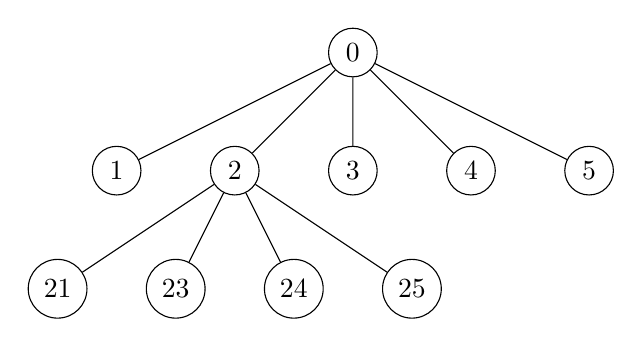
\begin{tikzpicture}[every node/.style={draw,circle}]
  \node (0) {0}
  child {node(1) {1}}
  child {node(2) {2}
    child {node(21) {21}}
    child {node(23) {23}}
    child {node(24) {24}}
    child {node(25) {25}}
  }
  child {node(3) {3}}
  child {node(4) {4}}
  child {node(5) {5}};
\end{tikzpicture}

The number of keys each node needs to keep will be increased
exponentially as $n - k$ is big. Up to $(10,7)$ threshold seems
practical.

\subsubsection*{DSA, ECDSA}
BFTKV implements a DSS threshold scheme introduced by Gennaro et
al. \cite{Gennaro}
Since the scheme has a restriction such that $n \geq 2t$ in the $(t,
n)$-threshold scheme, we no longer be able to use the quorum threshold
for $(t, n)$. But, we follow the protocols between the client and a
quorum, i.e., the client sends a signing request to a quorum
(multicast the message to all quorum members), then collect the
responses. Our signing protocol consists of three phases:
\begin{enumerate}
\item Collect joint shared secrets generated by each quorum member
\item Distribute the secrets to the quorum and calculate
  $r=g^{k^{-1}} \bmod p \bmod q$ where $k$ is the
  joint Shamir's shared secret (i.e., $k = \sum k_i$)
\item Distribute r to the quorum and calculate $s=k(m+xr) \bmod q$
  from each $s_i=k_i(m+x_ir) \bmod q$ returned from each quorum member
\end{enumerate}

\section{Protocols}

The system uses Phalanx \cite{Delhi:2} for the underlying {\em
read/write} operations. To maintain a graph for the quorum system, we
extend the protocols with {\em join/leave}. Also {\em register}
protocol is used to get quorum certificates with the threshold
password authentication.

\begin{quote}
  {\em Notations}:
  $\langle x, t, v, s_C, S \rangle$ is an ordered set that denotes the protocol
  data. $s_C$ and $S$ can be omitted.
  \begin{itemize}
  \item[$x$] is the variable and an arbitrary length octet string. The variable will
    be the key on the key-value store.
  \item[$t$] is the timestamp and a 64-bit non-negative integer. $2^{64}-1$ is
    a special value to denote that the variable is no longer able to be
    updated.
  \item[$v$] is the value and an arbitrary length octet string.
  \item[$s_C$] is an object of the signature and quorum certificate of a
    client $C$. $s_C.sig$ is the signature over $\langle x, t, v \rangle$ signed by the
    private key of $C$. $s_C.cert$ is the quorum certificate of
    $C$. $s_C.cert.ID$ is the unique ID to identify each node.
  \item[$S$] is an unordered set of the signature object. Each $S_i
    \in S$ has the
    same structure of the $s_C$. The signers must be quorum members.
  \end{itemize}
\end{quote}

\subsection{Read / Write}
\label{rw}
{\em read/write} protocols are done between a client ($C$) and a
quorum ($Q$). A quorum is chosen from a quorum system ($QS \subseteq
2^U$) which is a subset of the powerset of all nodes ($U$).  To write
a value $v$ into a variable $x$, we follow the write protocol
specified in Phalanx.\\

[ Write ]
\begin{align*}
  C :& \text{ choose a quorum from quorum cliques} \\
     & Q \in QC \\
  C \rightarrow Q :& \text{ {\em get timestamp}}(x) \\
  C \leftarrow Q_i :& \text{ } t_i \\
  C :& \text{ collect } 2b+1 \text{ timestamps: } \\
     & \text{ } \{t_i\}_{i \in \mathcal{T}}, |\mathcal{T}|=2b+1,
       \mathcal{T} \subseteq Q \\
  C :& \text{ choose the maximum timestamp } \\
     & \text{ } t = max(t_i) + 1 \\
  C \rightarrow Q :& \text{ {\em get signature}}(\langle x, t, v, s_C \rangle),\\
     & \text{ where } s_C = (Sign_C(\langle x, t, v \rangle), Cert_C) \\
  Q_i :& \text{ verify $s_C$ with $C$'s quorum certificates} \\
  Q_i :& \text{ check the TOFU policy} \\
  C \rightarrow Q_i :& \text{ } S_i = \{\langle x, t, v, s_C \rangle\}_{Q_i} \\
  C :& \text{ collect signatures } \\
     & \text{ } S = \{S_i\}_{i \in \mathcal{T}} \\
  C :& \text{ choose a quorum from } Q' = U \setminus QC \\
  C \rightarrow Q' :& \text{ write}(\langle x, t, v, s_C, S \rangle) \\
  Q'_i :& \text{ verify the signature set $S$} \\
  Q'_i :& \text{ do the equivocation check} \\
  Q'_i :& \text{ store } \langle x, t, v, S_C, S \rangle
\end{align*}

[ Read ]
\setcounter{equation}{0}
\begin{align*}
  C &: \text{choose a quorum } Q \in U \setminus QC \\
  C \rightarrow Q &: read(x) \\
  C \leftarrow Q_i &: M_i = \langle x, t, v, s_C, S \rangle \\
  C &: \text{collect } f + 1 \text{ responses} \\
  C &: \text{verify the signature set $S$} \\
  C &: \text{do the equivocation check} \\
  C &: \text{choose the latest timestamp } \\
    & t_L = max(M_i.t) \\
    & [ write back ] \\
  C &: Q' = \{Q_i \subset Q | M_i.t < t_L\} \\
  C \rightarrow Q' &: \text{{\em write back}}(\langle x, t_L, v, s_C, S \rangle)
\end{align*}


\subsection{Join / Leave}
Any node can join / leave anytime by sending its quorum certificate to
nodes it trusts. The node received the request verifies the
certificate and adds it to the local graph which will be returned to
the caller node. To leave the network, a node broadcasts its quorum
certificate to the quorum it belongs to.
The node that has received the graph constructs its own local graph
from the graphs, then sends the join request to nodes that have not
been connected.

\begin{algorithm}
  \caption{Join}
  \SetAlgoNoLine
  \KwIn{Cert}
  $G.V = Cert.sigs[].cert$\;
  $peers = G.V$\;
  \For{$peers = \bot$}
  {
    \For{$peer \in Peers$}
    {
      Send $Cert$ to $peer.ID$\;
      $certs = $ Receive()\;
      $peers = certs \setminus G.V$\;
      $G.V = G.V \cup certs$\;
    }
  }
\end{algorithm}

\subsection{Register}
\label{register}
Each node generates its own public/private key pair, then send the
public key part to a quorum to get a quorum certificate. Each quorum
member keeps all certificate issued to clients along with a partial
password secret. If it finds a certificate request that has the same
ID as one of the stored certificates it will sign it only if the
password authentication is done. The client will get a ``proof'' of
the authentication when it is finished.

\begin{algorithm}
  \caption{Register}
  \SetAlgoNoLine
  \KwIn{$req$: a client certificate, $proof$: the proof of the password
    authentication}
  $found$ = $Store[req.ID]$\;
  \If{$found \neq \bot$}
  {
    $clique = FindMaximalClique(self)$\;
    \If{$proof \subseteq clique$ {\bf and} $|proof| \ge
      |clique|\cdot2/3$}
    {
      $Sign(req)$\;
    }
  }
\end{algorithm}

\section{Security Analysis}
We look into attacks against the fundamental property:
$READ(Q_1,x) = READ(Q_2,x)$ for $\forall Q_1, Q_2 \in QS$, which is
known as equivocation.  The best that attackers can do is divide a
clique into two sets and ask each set to sign $\langle x,t,v \rangle$
and $\langle x,t,v' \rangle$ separately. Then do the {\em write}
protocol for the target nodes with collected signature sets $S$ and
$S'$. Honest servers will refuse the request because it does not
satisfy the basic $b$-masking quorum condition: $|S| \geq b+1$. But
with $b$ colluding nodes, the attack will succeed.

\newcommand{\slice}[4]{
  \pgfmathparse{0.5*#1+0.5*#2}
  \let\midangle\pgfmathresult

  % slice
  \draw[thick,fill=black!10] (0,0) -- (#1:1) arc (#1:#2:1) -- cycle;

  % outer label
  \node[label=\midangle:#4] at (\midangle:1) {};

  % inner label
  \pgfmathparse{min((#2-#1-10)/110*(-0.3),0)}
  \let\temp\pgfmathresult
  \pgfmathparse{max(\temp,-0.5) + 0.8}
  \let\innerpos\pgfmathresult
  \node at (\midangle:\innerpos) {#3};
}

\begin{tikzpicture}[scale=1.5]

\newcounter{a}
\newcounter{b}
\foreach \p/\t/\l in {25//,40/$H_1$/Honest nodes, 20/$F$/Faulty nodes,
40/$H_2$/Honest nodes}
  {
    \setcounter{a}{\value{b}}
    \addtocounter{b}{\p}
    \slice{\thea/100*360}
          {\theb/100*360}
          {\t}{\l}
  }

\end{tikzpicture}

The maximum number of signatures dishonest clients can get is
$b+(n-b)/2$. Therefore, to overcome the attack we need
\[ n-b > b+(n-b)/2 \Rightarrow n > 3b \]

\subsubsection*{Detecting equivocation on read}
Even if the number of faulty nodes exceeds the above threshold, the
system can detect malicious actions with the following probability
\begin{align*}
  F_p &= Pr[Q \cap H_1 \neq \emptyset \wedge Q \cap H_2 \neq
        \emptyset] \\
      & = 1 - Pr[Q \subseteq F \cup H_1] \\
      & = 1 - ((n + f) / 2n)^{|Q|}
\end{align*}
when $f > b$ and $|Q| < (f + n)/2$, where $f$ is the number of the
faulty nodes, assuming the sizes of $H_1$ and $H_2$ are the same.

In the case of $f \le b$ the detection rate is always 100\% because it is
guaranteed that clients can always find a valid value and anything
other than that is the result of malicious actions. When the number of
faulty nodes exceeds the threshold, i.e., $f \geq b$, it will be possible that
the client cannot detect all malicious actions. Since the minimum
quorum size is $(n-1)/3$ it does not need to consider the case where
$|Q| < n/3$. Also, if the size exceeds $(f+n)/2$ any quorum always
includes at least one node from each $H_i$ which makes the detection
rate 100\%. \\

\begin{tikzpicture}[xscale=6,yscale=6]
  \draw [<->] (0,0.9) -- (0,0) -- (1.0,0);
  \node [below right] at (1,0) {$|Q|$};
  \node [left] at (0,{1-pow(17/300,0.7)}) {$1$};
  \node [left] at (0,0) {$0$};
  \node [below] at (0.3,0) {$n/3$};
  \node [below] at (0.7,0) {$(f+n)/2$};
  \draw[dashed, domain=0:0.3] plot (\x, {1-pow(17/300,\x)});
  \draw[thick, domain=0.3:0.7] plot (\x, {1-pow(17/300,\x)});
  \draw[dashed, domain=0.7:1.0] plot (\x, {1-pow(17/300,0.7)});
\end{tikzpicture}

For example, assume we choose a quorum $|Q| = 3b+1$ out of $n = 4b+1$,
which is the default setup of the kv quorum system, the detection rate
is 100\% up to $f = 2b$ failure nodes. \\

\begin{tikzpicture}[xscale=6,yscale=6]
  \draw [<->] (0,1.05) -- (0,0) -- (1.05,0);
  \node [left] at (0,1) {$1$};
  \node [left] at (0,0) {$0$};
  \node [below] at (0.3,0) {$n/3$};
  \node [below] at (0.7,0) {$2n/3$};
  \node [below] at (1,0) {$n$};
  \node [right] at (1.05,0) {$f$};
  \draw[thick, smooth] (0,1) to (0.6,1) to [out=0,in=90] (1,0);
\end{tikzpicture}

\section{Applications}

We discuss some potential appliations of BFTKV.

\subsection{Decenteralized PKI with DKMS}

User authentication is a long-standing problem for end-to-end
systems. Even if we have semantically secure cryptographic protocols
to exchange data between users, if it was with a wrong one, the whole
security system would not make sense. On the other hand, once we have
a robust user authentication scheme, we can build up many kinds of
security systems on top of that, such as PGP and Signal. Our goal is
to construct an infrastructure to exchange public keys that represent
users' identities. Exchanging public keys can be done in person,
using a QR code, confirming the fingerprint of public keys, etc. Those
methods seem to be relevant for some situations, such as sending
money. Also, public key infrastructures using central authorities,
such as X.509 which is based on chain of trust, are widely used. A PKI
like X.509, however, still have a problem when issuing a certificate
to each end user. CAs issue certificates to corporates, organizations,
and individuals based on trustworthiness of requesters but for end
users whose authenticity is not easy to be proven, we have the same
basic issues. From end users' point of view, blindly relying on a
central authority based on its authenticity is no longer secure and
contradict the end-to-end philosophy.

Our proposed PKI does not ``strongly'' rely on central authorities,
yet it does not require to exchange public keys in person. Here are
the high level system requirements:
\begin{itemize}
\item Scalability -- the system can grow without affecting the current running services
\item Transparency -- anyone can monitor every system activity
\item Quantifiability -- security and efficiency can be formally analyzed
\item Robustness -- the system has to recover from erroneous situations by itself
\item Privacy -- the system should not reveal unnecessary information about users
\item Non-interactivity -- a client may not be able to interact peers
before sending a message. This particular requirement makes it
difficult to design a system that guarantees the ``what I saw is what
you see'' concept. SMTP, for example, is not a mutual explicit
authentication protocol. When an email is encrypted then sent out, if
it is encrypted with a wrong key, it will be too late -- someone in
the middle could read the email when the recipient receives the email
and notice that the encrypted email is not actually for her.
\end{itemize}

\subsection{As a consensus mechanism for Blockchain technologies}
Key-value stores can be suitable to store transactions. Without
knowing the key it will be difficult to access the value -- in this
sense it can be less transparent than other ledgers such as hash
chain. Once a transaction gets a collective signature, the transaction
can be stored in any way. The only concern is how to know a
transaction is latest. Each transaction has the timestamp and we can
easy get the latest $\langle x, t, v \rangle$ corresponding to $x$
{\em in a node} but we do not know if other nodes might have a newer
value. BFTKV addresses this issue by the simple quorum system -- as
long as $\forall Q_1, Q_2 \in QS, |Q_1 \cap Q_2| > f$, at least one
node in a quorum has the latest value and the client will choose the
one. This method is simple but it is difficult to scale out. We need
to collect data from $n - f$ nodes. Another way to address the issue
is to use epoch...

\section{Future Work}

Scalability of bitcoin blockchain is excellent -- you can add as many
nodes as you want and it will not affect the whole system, but the
latency and throughput of the whole process is terrible -- it takes
one hour to settle a transaction.
On the other hand, BFT type of blockchain settles transactions in a
range from sub milliseconds to a few seconds, but scaling out is
difficult. Specifically, with quorum systems we have theoretical lower
bounds such as $n = 3f + 1$ and we cannot do anything about it. Even
if the computational complexity is linear ($O(n)$) it is not realistic
to have tens of thousands nodes which is the number of the current
bitcoin nodes. 

One of the ideas to scale out the method is to use a threshold
signature to combine the set of quorum signatures so that each node
verifies the signature only once. But we need a dealer for the
threshold signature scheme and it will contradict the decenteralized
concept and make the system less flexible.

\begin{thebibliography}{99}

\bibitem{bitcoin}
  Satoshi Nakamoto (2008) Bitcoin: A Peer-to-Peer Electronic Cash System

\bibitem{Delhi:1}
  Malhi, D. and Reiter, M. (1998). Byzantine Quorum Systems

\bibitem{Delhi:2}
  Malhi, D. and Reiter, M. (1998). Secure and Scalable Replication in Phalanx

\bibitem{Gennaro}
  Gennaro, R., Jarecki, S., Krawczyk, H. and Rabin, T. (1999). Robust
  Threshold DSS Signatures

\bibitem{shoup}
  Shoup, V. Practical Threshold Signatures
  
\bibitem{srp}
  Wu, T. (2000). The SRP Authentication and Key Exchange System (RFC
  2945)

\end{thebibliography}

\end{document}
